\subsection*{Three tiers of annotation in a whole genome}
% Condensed version: one table, one listing, one figure, about 650 words.

Annotation sources change at different rates, and vepyr handles them with
three mechanisms (Table~\ref{tab:cTiers}): the core cache, which follows
Ensembl releases; plugin caches, which follow their providers; and ad hoc
sources, which a particular analysis needs and which are read from their
URLs when the query runs, without a build step. We applied all three to the
GIAB HG002 benchmark call set (NIST v4.2.1, chromosomes 1--22,
\NVariants{} variants after decomposition) to ask which genes a healthy
individual inactivates, whether selection against such variants is visible
in a single genome, which clinically classified variants HG002 carries and
from which parent, and in which disease genes a negative result would be
uninformative.

\begin{table}[ht]
\centering\small
\newcolumntype{L}[1]{>{\raggedright\arraybackslash}p{#1}}
\begin{tabular}{L{0.12\textwidth}L{0.38\textwidth}L{0.13\textwidth}L{0.27\textwidth}}
\toprule
Tier & Data used here & Updated & Mechanism \\
\midrule
1 Core cache & Ensembl~116: consequences, HGVS, MANE, gnomAD frequencies (incl.\ Ashkenazi Jewish) & with Ensembl releases & \texttt{build\_cache()}; read by \texttt{annotate()} \\
2 Plugin caches & ClinVar (2026-07-06), SpliceAI, AlphaMissense, CADD~v1.7 & weekly to yearly & \texttt{build\_plugin\_cache()}; matched by \texttt{annotate()} \\
3 Ad hoc sources & gnomAD~v4.1 gene constraint; ClinGen gene--disease validity; Ensembl~116 GFF3; GIAB v3.6 stratifications; v4.2.1 benchmark regions and VCFs of HG002 and both parents (\NRemoteSources{} files, \RemoteRows{} million records) & per analysis & read by URL with polars-bio (BED over HTTPS, VCF from S3) or Polars; joins, \texttt{overlap()}, \texttt{coverage()} \\
\bottomrule
\end{tabular}
\caption{Tiers of annotation in the HG002 analysis. Tiers 1 and 2 took
\AnnotateSec\,s for \NVariants{} variants (\Workers{} workers, Apple M3
Max); reading all tier-3 sources took \RemoteSec\,s.}
\label{tab:cTiers}
\end{table}

The analysis is a single Python script; the listing shows its structure
(abridged; the complete code is in \texttt{paper/hg002-tiered-annotation}):
\begin{lstlisting}[language=Python]
lf = vepyr.annotate("HG002_v4.2.1.split.vcf.gz", "vepyr_cache/116_GRCh38_ensembl",
                    reference_fasta=FASTA, workers=8,                     # tier 1
                    plugin_cache_root="vepyr_plugin_cache",              # tier 2
                    plugins=["clinvar", "alphamissense", "spliceai", "cadd"])
lf.select(*COLUMNS).sink_parquet("HG002.parquet")
mane = (pl.scan_parquet("HG002.parquet").with_row_index("vid")
          .explode(CSQ_LIST_COLUMNS, empty_as_null=True)
          .filter(pl.col("MANE_SELECT").is_not_null()).collect())
plof = mane.filter(pl.col("Consequence").str.contains(
    "stop_gained|frameshift_variant|splice_acceptor_variant|splice_donor_variant"))
# tier 3: read from the URLs when the query runs
segdups = pb.scan_bed(f"{GIAB_STRAT}/SegmentalDuplications/GRCh38_segdups.bed.gz")
benchmark = pb.scan_bed(HG002_BENCHMARK_BED)                 # HTTPS
father = pb.scan_vcf(f"s3://giab/release/AshkenazimTrio/{HG003_VCF}",
                     info_fields=[], format_fields=["GT"])
constraint = pl.scan_csv(GNOMAD_V41_CONSTRAINT_TSV, separator="\t", infer_schema=False)
in_segdup = pb.overlap(plof, segdups, overlap_output="left", distinct_output=True)
callable_bp = pb.coverage(mane_cds, benchmark)          # per CDS interval
\end{lstlisting}

\paragraph{Loss of function.} Of \NPlof{} variants with a stop-gained,
frameshift or canonical splice-site consequence in a MANE Select
transcript, \NHc{} in \NHcGenes{} genes pass filters drawn from all three
tiers (Figure~\ref{fig:cSummary}a). Tier~1 removes premature stops in the
last exon, which escape nonsense-mediated decay, and alleles with a gnomAD
frequency of at least 95\%: the \textit{FMO2*2} stop that inactivates
\textit{FMO2} in most humans and pairs of frameshifts in \textit{SON} and
\textit{SLAIN1} that restore the reading frame where GRCh38 carries a rare
sequence. Tier~2 removes variants classified benign in ClinVar, such as
\textit{LPL} p.Ser474Ter (S447X), and splice-site variants without SpliceAI
support. Tier~3 removes variants in segmental duplications or
low-mappability regions, such as the \textit{CYP2D6*4} splice variant, and
premature stops covered by the 50-bp rule. pLoF variants are depleted from
genes intolerant to LoF: \LoeufAllPlofPct\% lie in the two lowest gnomAD
LOEUF deciles, against \LoeufSynPct\% of rare synonymous variants
($p=\LoeufAllPlofP$; Figure~\ref{fig:cSummary}b), the signature of
purifying selection in one genome.

\paragraph{Clinically classified variants and inheritance.} The only ClinVar
pathogenic or likely pathogenic variant with review criteria is
\textit{\PlpGene} \PlpHgvsp{} (Glu117Ter in legacy numbering), the
Ashkenazi founder allele of factor~XI deficiency, heterozygous in HG002. Its
gnomAD frequency is \PlpAsj\% in Ashkenazi Jewish samples and \PlpAf\%
overall, and the father's VCF, streamed from S3, shows that it was inherited
from him. The parental VCFs resolve the origin of 9 of the \NHcRare{} rare
high-confidence pLoF variants and show that the only homozygous one, a
45-bp deletion of the \textit{PEX5} exon~2 donor that is absent from gnomAD,
is homozygous in both parents; with an alternative in-frame donor 45\,bp
downstream, it is most probably not a loss of function.

\paragraph{What cannot be seen.} \texttt{coverage()} of MANE Select coding
sequence by the benchmark regions shows that \NClinGenLtNinety{} of
\NClinGenGenes{} ClinGen disease genes have less than 90\% of their coding
sequence assessable (Figure~\ref{fig:cSummary}c), mostly in GIAB difficult
regions; they include \textit{CBS}, which lies in a falsely duplicated
region of GRCh38. A negative result in these genes is not informative.

\paragraph{Performance.} Annotation of the whole genome with the core cache
and four plugin caches took \AnnotateMin\,min; everything else, including
reading the twelve ad hoc sources, took \AnalyzeMin\,min, in one Python
process and without intermediate VCF, BED or index files. Changing a
tier-3 question---another gene set, stratification or relative---changes a
URL, not a cache.

\begin{figure}[ht]
\centering
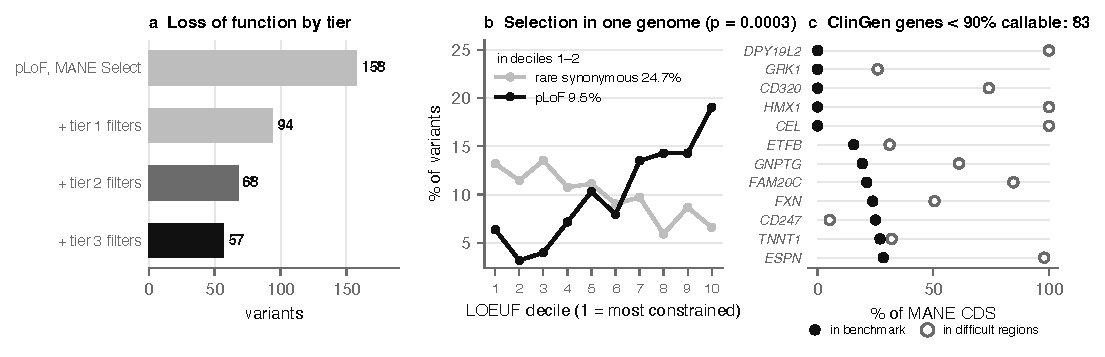
\includegraphics[width=\textwidth]{figures/figS_hg002_summary.pdf}
\caption{Three tiers of annotation in the HG002 genome. (a)~Variants with
a MANE Select pLoF consequence remaining after the filters of each tier.
(b)~Distribution of pLoF and rare synonymous variants across gnomAD v4.1
LOEUF deciles; the legend gives the share in the two most constrained
deciles ($p$, Fisher's exact test). (c)~The twelve ClinGen genes with the
smallest share of MANE Select coding sequence in the HG002 benchmark
regions, and the share in GIAB difficult regions.}
\label{fig:cSummary}
\end{figure}
